
\chapter{Padding Oracle Attack}
\label{chapter:POA}

Cette attaque a pour objectif de retrouver le clair d'un bloc chiffré 
avec le mode CBC. Elle s'appuie sur le fait que le dernier bloc chiffré
contient du padding. De plus le dernier octet de padding corespond à la
taille du padding.\\
L'oracle  déchiffre le clair et vérifie que la taille du padding est correcte. 
Il renvoie une erreur en cas de taille erronée.\\

\begin{figure}[h]
\label{fig:cbc}
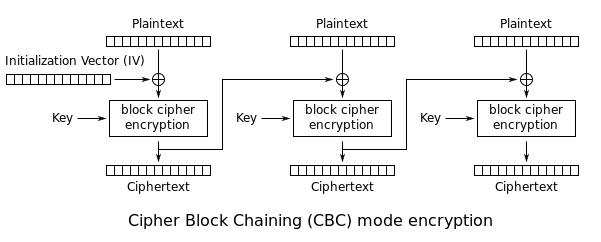
\includegraphics[scale=0.5]{CBC_Encrypt}\\
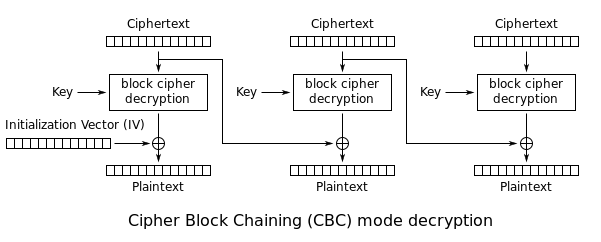
\includegraphics[scale=0.5]{CBC_Decrypt}
\caption{Schéma du Mode CBC}
\end{figure}

Supposons maintenant que l'attaquant posséde un chiffré composé de 4 blocs :
$C_1||C_2||C_3||C_4$. Le bloc $C_4$ contient un padding de taille $x$ connu par l'attaquant.
il souhaite connaitre le contenu de $C_2$ et quand il interoge l'oracle, celui-ci lui dit
si la taille est correcte ou non.\\
L'attaquant peut envoyer une version contrefaites du chiffré comme suit :
$C_1||C_2||C_3'||C_4'$.\\
\begin{itemize}
\item le bloc $C_4'=C_2$
\item le bloc $C_3'= C_3$ dont le dernier octet est modifié
\end{itemize}
Soit $P_n$ le déchiffrement de $C_n$ par l'oracle et D() et E() les algorithmes
de déchiffement et de chiffrement. 
Le bloc qui nous intérésse est $P_4'$.
\[P_4' = D(C_2) + C_3'\]
or $C_2 = E(P_2 + C_1)$ d'où

\[\Longleftrightarrow P_4' = D(E(P_2 + C_1)) + C_3'\]
\[\Longleftrightarrow P_4' = P_2 + C_1 + C_3'\]
\begin{itemize}
\item $C_1$ et $C_3'$ sont connus
\item $P_2$ est le clair recherché
\item $P_4'$ est inconnu mais l'oracle nous dit si le dernier octet égale à $x$.
\end{itemize}
Soit k la taille des blocs et Pn[i] le iéme octet du bloc n.

\[P_4'[k] = P_2[k] + C_1[k] + C_3'[k]\] si $P_4'[k] = x$ alors
\[\Longleftrightarrow x = P_2[k] + C_1[k] + C_3'[k]\]
\[\Longleftrightarrow P_2[k] = x + C_1[k] + C_3'[k]\]

Ce qui donne une equation a une seule inconnu donc l'attaquant a trouvé $P_2[k]$.
Pour avoir $P_4' = x$, il suffit de faire varier la valeur de $C_3'[k]$. Il est donc
possible de trouver le dernier octet de $P_2$ en maximum de 256 essais.\\

Pour trouver les autres octets, l'attaquant prend $P_4'[k] = P_2[i]$ où $i \in [1,k]$.
Avec cette méthode il est possible de retrouver tout le contenu d'un chiffré à
l'exeption du premier bloc (sauf si l'IV est connu).\\

Cette attaque n'est pas utilisable tel quel sur SSL car elle demande de modifier un octet
d'un bloc qui n'est pas du padding. Cela entraine un échec du déchiffrement du bloc, le
paquet sera donc rejeter à la vérification avec la MAC. Elle est toutefois le point de
départ de nombreuses attaques sur SSL/TLS dont Poodle~\ref{part:poodle}.
